\documentclass{article}
\usepackage[utf8]{inputenc}

\usepackage{indentfirst}
\usepackage{url}
\usepackage{hyperref}
\usepackage{graphicx}
    \DeclareGraphicsExtensions{.png, .jpg, .jpeg}
    
\usepackage{wrapfig}
    
\usepackage{biblatex}
\addbibresource{P2_Team_03.bib}

\title{CS791 Project 3: Experimental Setup \\ A Usability Evaluation of a Public Collaborative Data Portal, an Update}
\author{\emph{Team 2}: Terence Henriod, Vinh Le \\ \emph{Instructor}: Sergiu Dascalu}
\date{\today}

\begin{document}

\clearpage            % necessary for removing page number on first page

\maketitle
\begin{center}

\includegraphics[scale=0.4]{unr-logo} \\[0.5cm]
\textsc{\Large University of Nevada, Reno} \\[0.5cm]
\textsc{\large Computer Science and Engineering Department} \\
\end{center}

\thispagestyle{empty} % removes the page number from the title page

% create some whitespace between title stuff and abstract
\vspace{10mm}

%
%
\newpage
\section{Introduction}
The NRDC grown exponentially over the past two years; its initial user base started with a select few individuals and has grown to accommodate almost three thousand users. New services are added routinely as the system encompasses more and more projects. As development continues for the NRDC, it is vital that the current services are continually optimized for a better user end experience or else risk a loss of attraction in the eyes of its users. The idea of this project is to perform a user study on the main services present within the system in order to extrapolate a plausible future direction for the NRDC. In this user study, participants will be utilizing the already developed web services located on the NRDC, whilst providing feedback based on ease of usage. 

One of the main ideals that make up Human and Computer Interaction (HCI) is the pursuit or development of a better user end experience. As this study is designed to find that better experience, this project holds a great deal of relevancy to the field of HCI. The NRDC is heavily affiliated with the Department of Computer Science and Engineering (CSE), which allows for an easier access to references and support, thus making the choice of having this user study very attractive. Additionally, this study would benefit the members of the CSE department, as well as the National Science Foundation, making this a fantastic choice to give back to the both organizations, as we have been affiliated with them in the past.

In the end the final goal of this user study is to developed a more intuitive system, which balances pragmatism and a user friendly approach, for the services in the Nevada Research Data Center.

Since the original version of this document, some changes were made, many of them inspired by a test run of the experiment with out "test participant". This trial run helped us to see where participants would stumble, rethink the data we should collect, and take note of data and observations we should make that were not directly relevant to the original experiment.

%
%
\section{Revised Methodology}
%
\subsection{Participants}
In this user study, we will gather at least 6 participants (8 were gathered in total), all of whom will be students or researchers from the University of Nevada, Reno. The NRDC aims to provide data services to students and researchers aiming to complete research in the state of Nevada. In light of this, each of these participants will be members of a mainly research-oriented major, such as Computer Science and Engineering, Math, or Physics, in order to simulate a likely situation of usage as possible. These participants will have no experience with the system in question and minimal training will be issued in order to close any gap of skill in between participants (it is recommended that uninitiated users are actually good candidates for exposing usability difficulties\cite{dontmakemethink}). Participants will be recruited through affiliated graduate organizations, local philanthropy events, and various student organizations on campus. The experiment itself will be brief and refreshments will be offered as suitable compensation.

%
\subsection{Apparatus}

\subsubsection{NRDC}
The NRDC is the web interface itself that is the target of evaluation for this user study. The NRDC is a web portal containing various services that are linked on the main page of the NRDC itself. Both versions of the NRDC will be used, the version currently in deployment and the new one currently in development. The web services on the NRDC are: the WebCam Image Archive, the Geospacial Data Search, and Current Conditions. The WebCam Image Archive is a service that allows users to navigate to all of the current research sites affiliated with the NRDC. Users will have the ability to save, view, and download webcam images taken during a specified time each day. Additionally, users may also have these images stringed together to form a video with the option of downloading it. The Geo-spatial Data Search allows users to navigate to an affiliated research site through Google Maps and retrieve actual quantifiable data by narrowing down the the filter and dates. The Current Conditions provides users with the ability of retrieving live research data at a specified research site through Google Maps.

\subsubsection{Work Station}

\begin{wrapfigure}{r}{0.6\textwidth}
  \begin{center}
    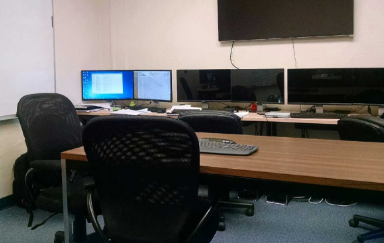
\includegraphics[width=0.48\textwidth]{ci_lab_apparatus}
  \end{center}
  \caption{The testing location: the UNR Cyber-Infrastructure Lab.}
\end{wrapfigure}

Users will use a typical Windows desktop workstation with a standard monitor, keyboard, and mouse. The workstation will be in a typical group office/workspace (the Cyber Infrastructure Lab, located in the Scrugham Engineering and Mines building, room 255, at the University of Nevada, Reno), which should afford participants a relatively calm working environment. This standard setup should be very comparable to the typical workspace used by typical NRDC users.

\subsubsection{Tasks and Data Collection}
Tasks will vary, and will include use of the NRDC's major services and links to various information.

\begin{figure}[h!]
  \centering
  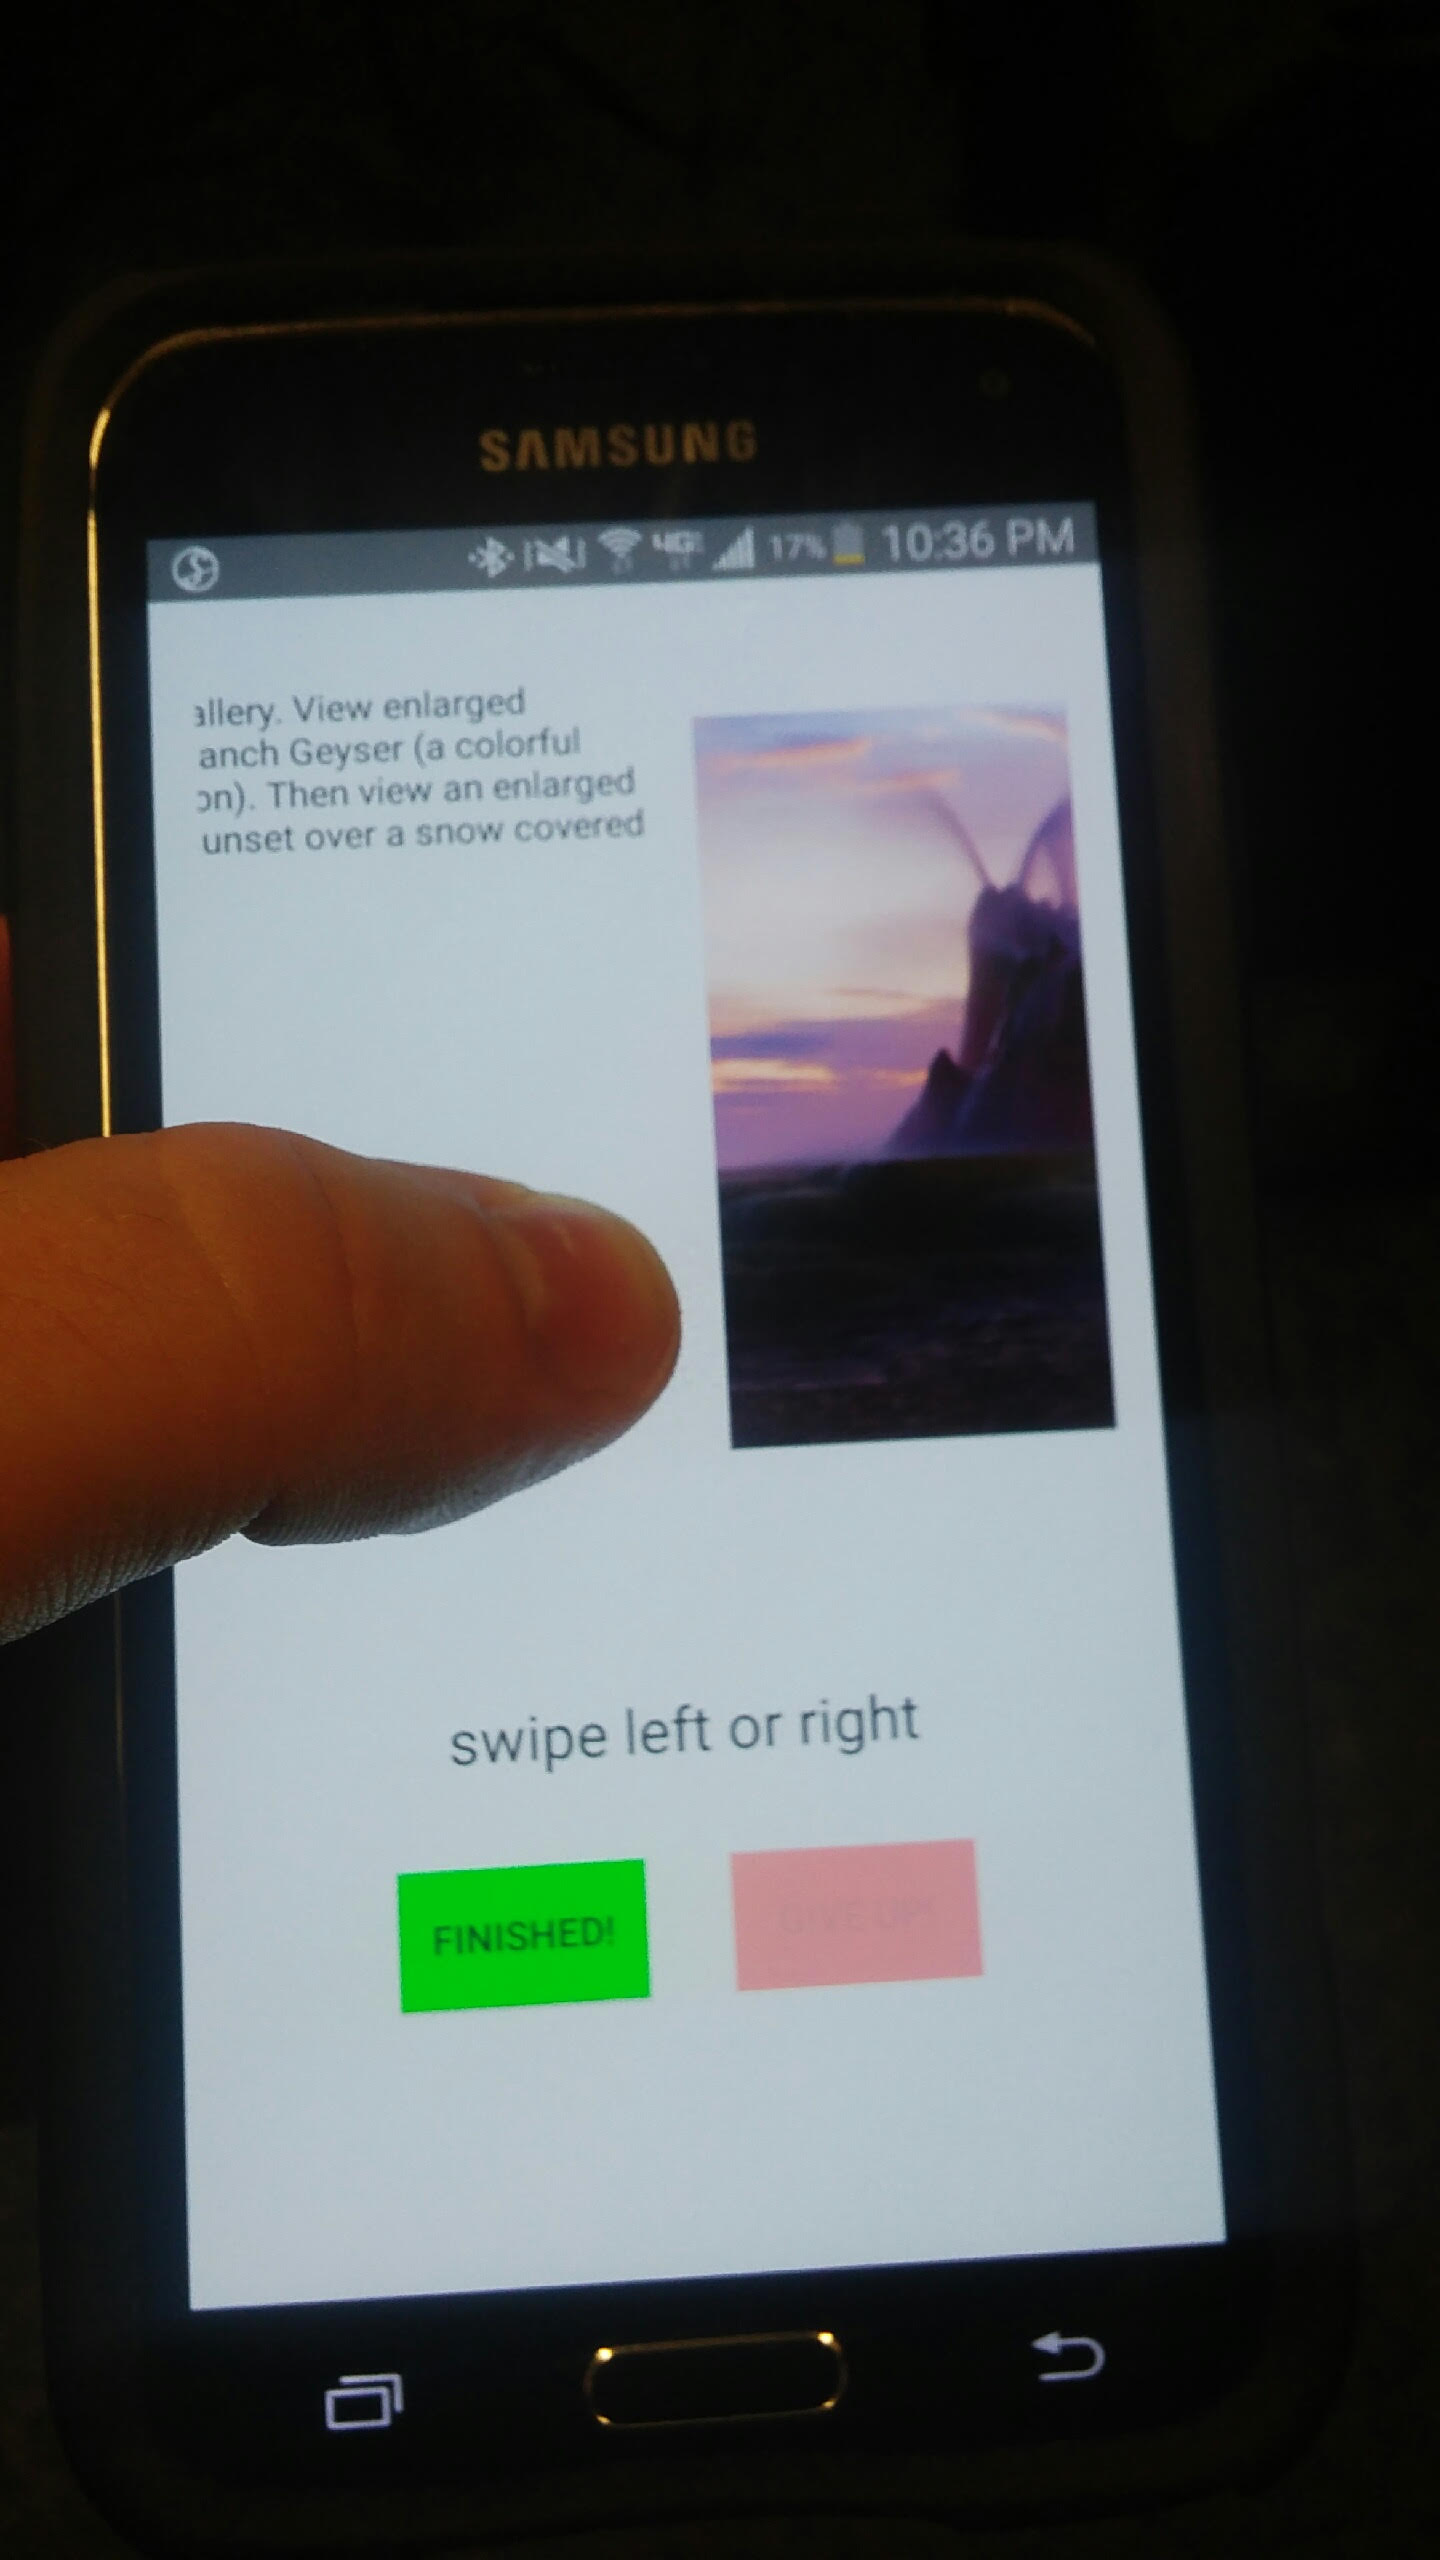
\includegraphics[width=.3\linewidth]{task_app}
  \caption{The task-dispensing app used to give participants tasks. In this image, the user is alternating between a text description of the task and a screen-shot of the desired result.}
  \label{fig:task_app}
\end{figure}

To present tasks and collect timings, a third-party mobile phone application, named \emph{HCI-Task}, will be used. This will be a simple Android application used on a 4+" touchscreen smart phone that will allow users to swipe between a text description of the task and a screen shot of the goal state for the task, as well as declare when a task has been completed or given up on.

Some data that is difficult to collect through software will be collected "manually" by the researchers. The researchers will also count clicks made by participants, their use of certain features of the NRDC, and record poignant observations of participant behaviors or remarks.

%
\subsection{Procedure}
The steps of the experiment will be conducted for each user as follows:
\begin{enumerate}
\item Participant will be greeted, and then given a brief description of what the NRDC, its purpose, and what the reason for conducting a user study is.

\item Participants will be directed to a workstation and briefly shown how to access the NRDC interface version they have been assigned to work with (which will be labeled in such a way as to not introduce bias as labels as words like "new" and "old" might).

\item Participants will be given the smart phone that will display the tasks that they are to complete, introduced to the NRDC interface they will be starting with, and walked through an initial training task. This will help mitigate the effects of participants being too unfamiliar with what the goals of the study are to be effective. Participants then complete 3 short tasks (dispensed by the app) to familiarize them with use of the app.

\item Participants will then complete 7 tasks on their own, as quickly as possible. The phone will display the task prompts and collect performance data. Users will be allowed to give up on tasks after 3 minutes if they feel frustrated or discouraged, at a point when they would naturally seek help from another person. Should a participant give up, they will be briefly shown how to correctly perform the task so as not to skew the results for future tasks.

\item A short break will be taken. The researchers will prepare for the next step, and possibly have casual conversation with the participant.

\item Participants will again be directed to complete another 7 tasks as quickly as possible, this time with the other NRDC interface. The tasks are completed in the same manner as before.

\item Participants will complete a survey composed of both Likert scale and open-ended questions regarding their subjective assessment, preferences, and suggestions about the NRDC and its interfaces.

\item Finally, participants will be debriefed, allowed to ask questions, and offered refreshments as compensation for their participation.
%
\end{enumerate}

%
\subsection{Tasks}
Participants will be asked to retrieve data from each of the major services that compose the NRDC, as well as locate information in the NRDC interface itself. The tasks will be timed to measure performance, but users will be given the option to "give up" on any task after 3 minutes to help measure search perseverance in tandem with task performance.

\begin{enumerate}
\item Geo-Spatial Data Search
The Geo-Spatial Data Search service provides a variety of data from several very specific locations in the Nevada wilderness. Participants will be asked to retrieve a specific set of (applicable) data from a specific location for a random time period in the past. Variables and locations will be determined ahead of time by the researchers, since not all types of data are available for all locations. This task will be considered complete once the participant has viewed the raw data.
    
\begin{figure}[h!]
  \centering
  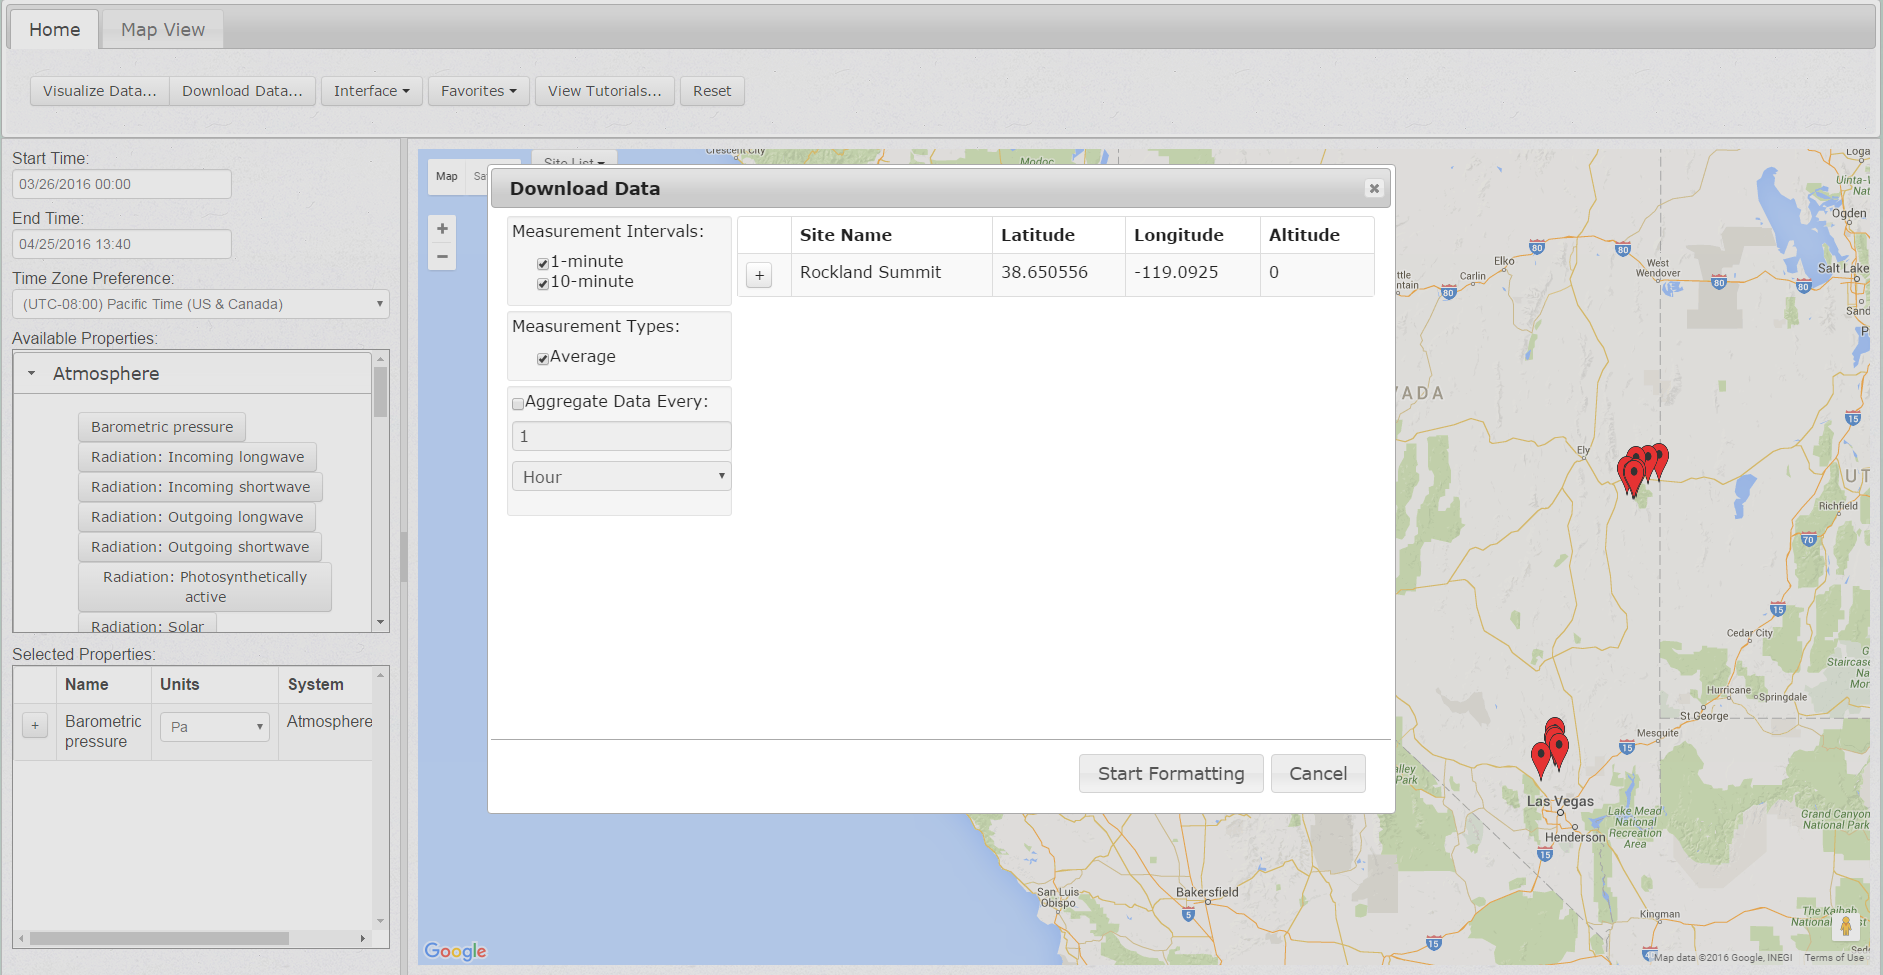
\includegraphics[width=.6\linewidth]{geospatial}
  \caption{A screen shot of some basic data obtained through the Geospatial Data Search.}
  \label{fig:geospatial}
\end{figure}

\item Webcam Image Archive
The Webcam Image Archive features real, sometimes scenic, imagery captured by remote cameras. Participants will be asked to retrieve a collection of images from a particular location and a particular date and time, determined by the researchers beforehand. This task will be considered completed once the participant has been able to scan through the selected image set to verify that it has been retrieved.

\begin{figure}[h!]
  \centering
  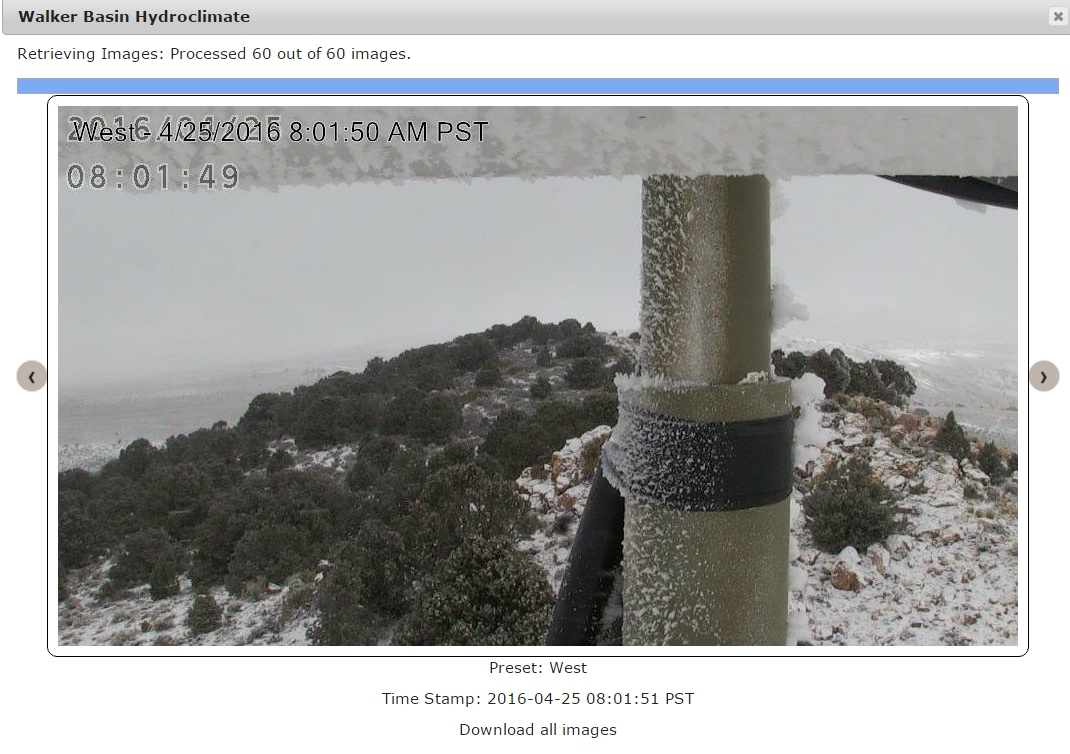
\includegraphics[width=.6\linewidth]{webcam-image-archive-example}
  \caption{A screen shot of the partial results from the a Webcam Image Archive task.}
  \label{fig:webcam-image-archive}
\end{figure}


\item Current Conditions
The Current Conditions service neatly summarizes much of the data for a given location, integrating weather data and a current webcam image. In order to evaluate both the navigability of this feature and the usability of the displayed data, participants will be asked to find the current conditions for a specific location and retrieve the values of two items of the displayed data. The location and which data items will be selected beforehand by the researchers. The task will be considered completed once the participant self-identifies as having found the requested information.

\begin{figure}[h!]
  \centering
  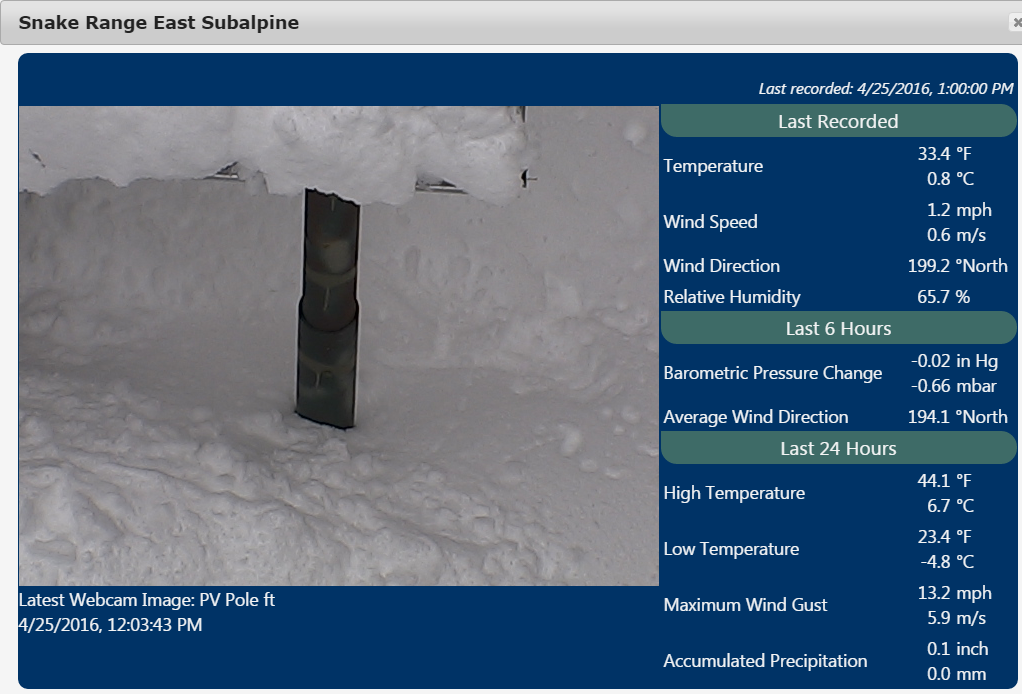
\includegraphics[width=.6\linewidth]{current-conditions-example}
  \caption{An sample screen shot of the Current Conditions interface.}
  \label{fig:current-conditions}
\end{figure}

\item Submissions
The NRDC has functionality to submit for review new data sources and research results. Participants will be asked to locate these mechanisms, and use them up to the point of submission to evaluate their locatability and ease of use.

\item Connections and Other Information
In addition to hosting various sources of data, the NRDC features connections to other projects and links to information about the NRDC itself. Participants will be asked to locate this kind of information as though they were a person interested in finding that type of data.

\item Subjective Analysis
After completing the primary tasks, participants will be asked to rate the NRDC interfaces (current and in-development) in terms of preference, ease of use, and suggestions for improvement. This task is unlike the others in that it is not traditional performance research task per se, nor it it directly related to the NRDC.

%
\end{enumerate}

%
\subsection{Design}
The user study will explore the effect of the version of NRDC interface on task completion performance and subjective response to the interface. The experiment will be a 1 x 2, mixed between- and within-subjects experiment. The experiment is a within-subjects design in that participants are exposed to both interfaces for subjective evaluation, but a between-subjects design in that participants can only be exposed to one interface first to capture/isolate the learning effect.

\subsubsection{Independent Variable}
The independent variable \emph{Interface Version} will have two levels: \emph{current} and \emph{in-development} (for participants they will be labeled as \emph{Interface 1} and \emph{Interface A} to prevent any biasing inferences). It should be noted that \emph{Interface Version} represents the interface that participants will have their performance measured on, as well as which of the two interfaces participants will encounter first for the subjective evaluation (although, in the second sense, we hope this will have no effect on any of the examined outcomes).

Technically, which task a participant completes could be considered an independent variable, but as we are not interested in the effects of different tasks for this experiment, we will treat the tasks separately from one another and almost as though performance on each task were it's own dependent variable.

\subsubsection{Dependent Variables}
The first dependent variable is \emph{Task Performance}, which will be measured in seconds. The second will be \emph{Task Effort}, which will be the count of mouse clicks that each participant requires to complete each task. Implicit in these variables is also \emph{Task Perseverance}, which will simply be a measure of when participants choose to end a task because they feel it is taking unreasonably long to complete. \emph{Task Perseverance} will be a count of how many times a participant "gives up", and will be analyzed if enough concessions are observed.

On the subjective side, \emph{Interface Preference} will be measured using Likert scale responses and collect open-ended feedback. \emph{Interface Preference} will actually be comprised of several variables - one for each survey question.

\subsubsection{Control Variables}
Control variables will include \emph{Work Setting} (which will be restricted to a small, communal university work space) and \emph{Work Station Type} (which will be restricted to a standard Windows desktop work station).

\subsubsection{Counterbalancing}
Due to the two-fold nature of the study, the evaluation of \emph{Task Performance} will be treated as a between-subjects study to eliminate the order-effect of participant learning, but the evaluation of \emph{Interface Preference} will be treated as a within-subjects due to the necessity of participants needing to experience both levels of \emph{Interface Version} to determine a preference.

In order to counterbalance the order-effect of participant preference of one interface or the other, participants will evenly divided between the two levels of \emph{Interface Version}. It is possible that \emph{Interface Version} will be a confounding variable, but we hope to prevent this by giving participants different tasks to complete with their second interface to try and preserve any of the novelty experienced when working with the first interface.

\subsubsection{Summary}
For the objective performance measurements, 8 participants x 2 rounds x 7 tasks x 3 measurements per task = 336 total measurements will be collected. For the purposes of the questionnaire, 8 participants x 12 questions = 96 total responses. This is a combined 432 measurements.

%
%
\section{Results}

Many results were obtained from the experiment; some directly useful for our immediate experiment goals, others more as feedback for the NRDC developers. 

The following tables, figures, and quotes come from the 8 participants and the thoughts had by the researchers during the experiments. The following is not an all-inclusive list, but a summary to give a general idea of the outcomes of the experiment (there is a lot of data to process and we are still deciding on the best course of action for presenting the data).

%
\subsection{Quantitative}

Data was collected both on the objective performance of participants and their subjective responses about their experience. Perhaps the most definitive results actually came from the questionnaire. These results showed a clear preference for the \emph{in-development} version of the NRDC, and indicated that development is headed in a good direction. However, improvements can still be made (as discussed in the qualitative results section).

\subsubsection{Subjective Responses}
Participants clearly preferred the \emph{in-development} version of the interface, at least weakly, but strongly in most cases. The \emph{in-development} version seems to be best suited for work involving using all of the NRDC's resources and for uninitiated users (we can say this based on both the participants' responses to Q4 of the direct comparison, but also based on their general preference with the participants themselves being uninitiated users).


\begin{figure}[h!]
  \centering
  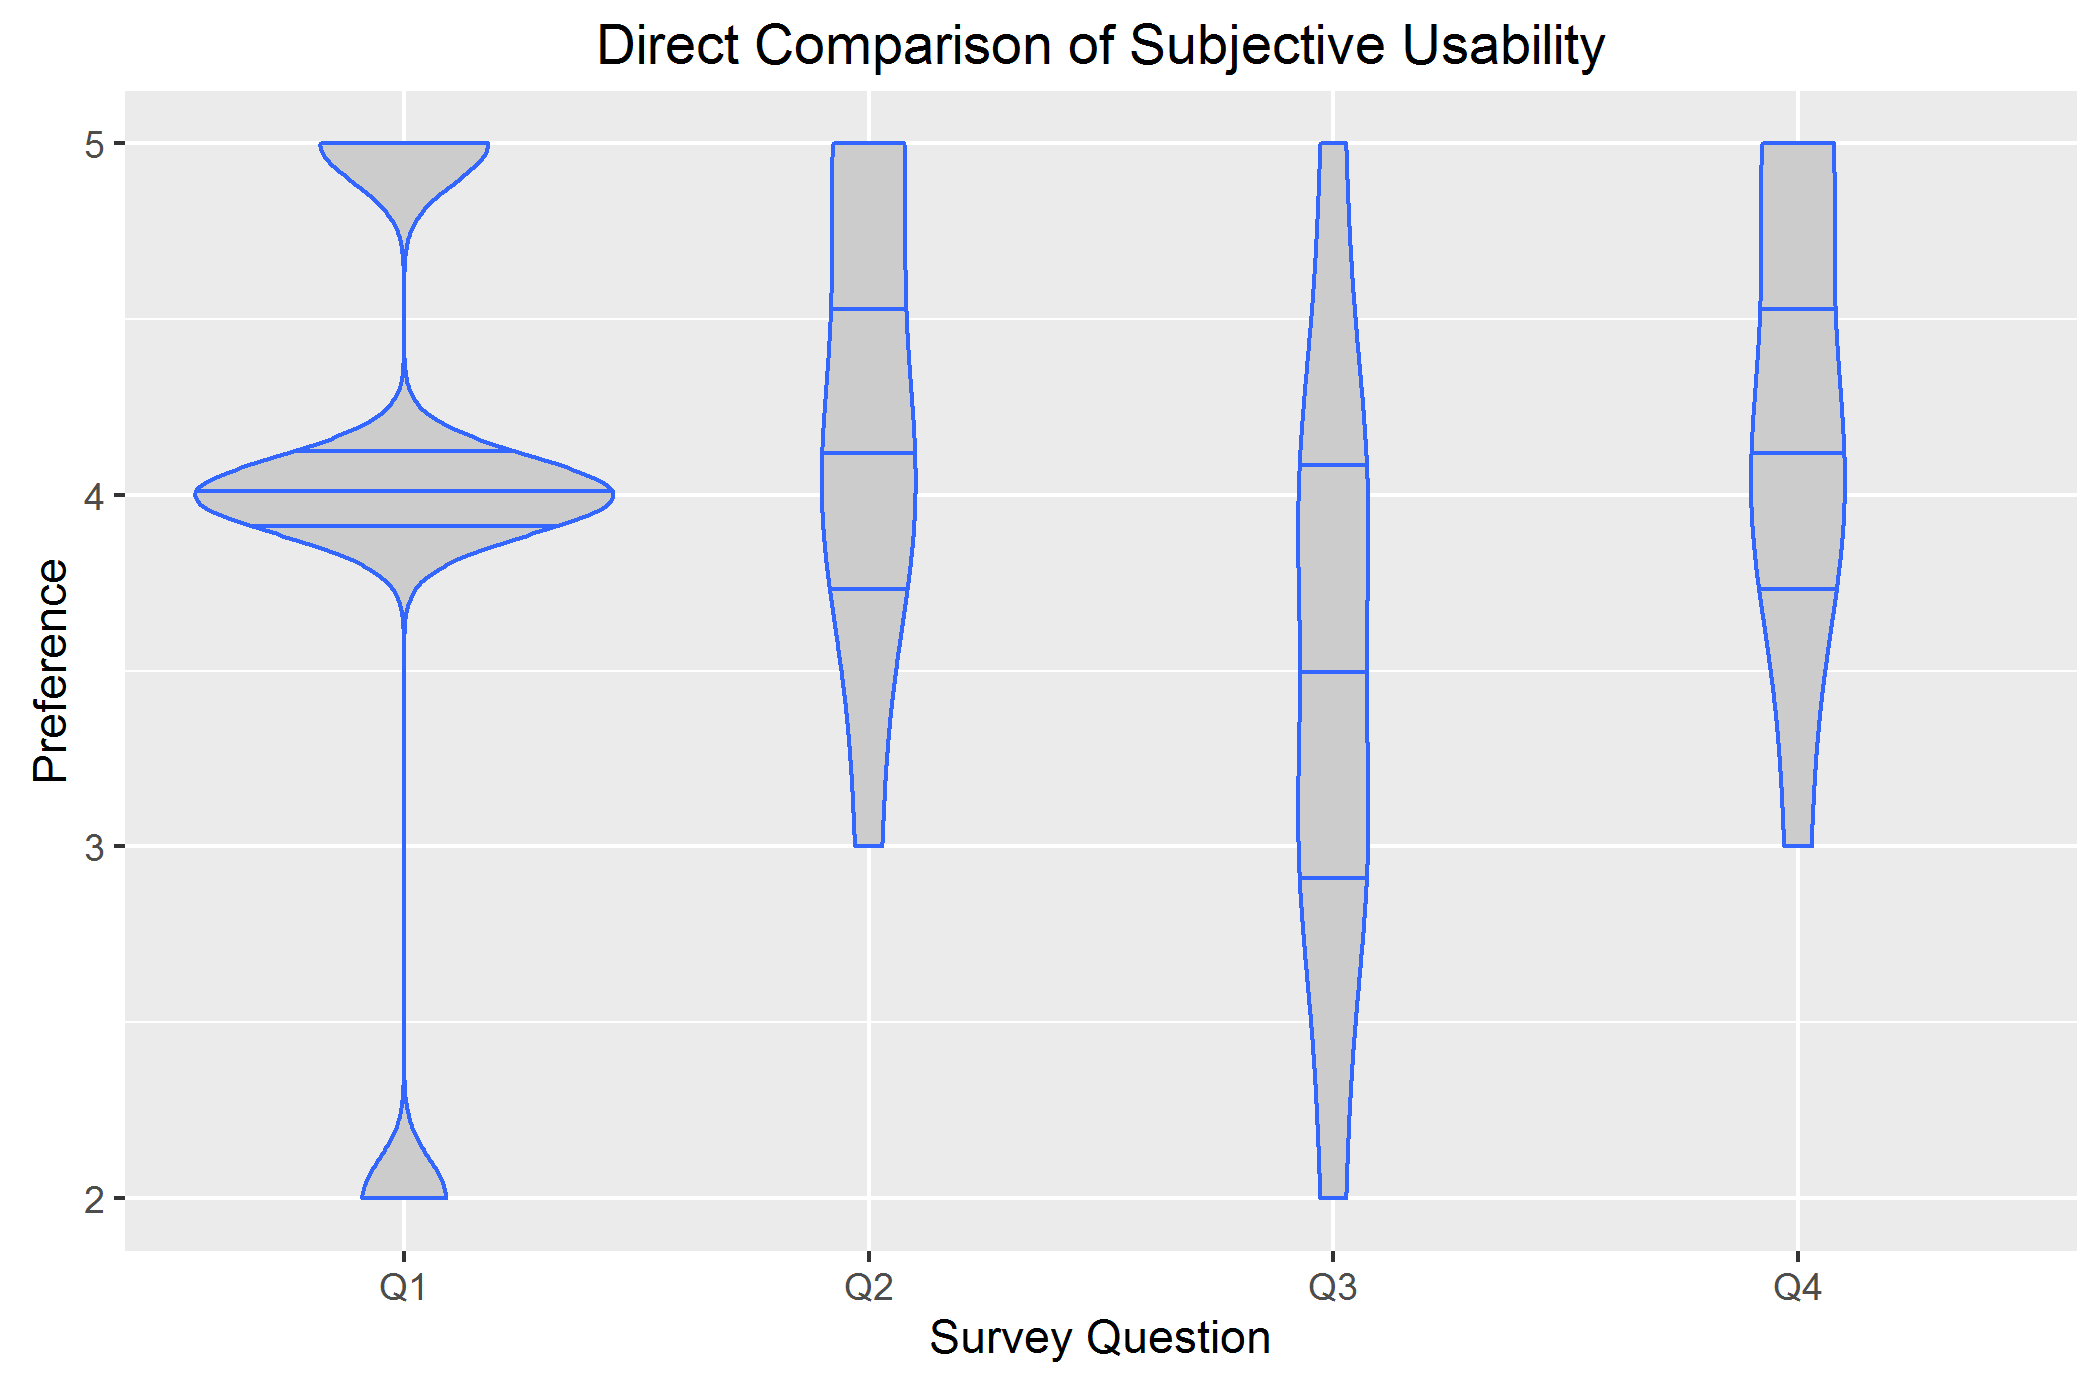
\includegraphics[width=.6\linewidth]{direct_comparison_violin}
  \caption{A violin plot indicating the distribution of responses. The plot is wider at sections where there were more responses with that value.}
  \label{fig:subjective_direct}
\end{figure}

In general, we see that participants did vary somewhat in their responses, but actually varied little when declaring an overall preference between the two interface versions.

\begin{table}[h]
    \centering
    \begin{tabular}{| c | p{4cm} || c || c | c | c |}
    \hline
    \multicolumn{6}{|c|}{Direct Comparison of Interface Versions} \\
    \multicolumn{6}{|c|}{(1 - current; 5 - in-development)} \\
    \multicolumn{2}{|c||}{Survey Question} & Preference & Significant (Y?) & $p$-Value & $F$-Value \\
    \hline
    \hline
    Q1 & Overall preference between interfaces &
    4.00 & Y & 7 e-4 & 18.667 \\
    \hline
    Q2 & Working with the NRDC, working between multiple services, switching regularly &
    4.25 & Y & 5 e-6 & 50 \\
    \hline
    Q3 & Working with the NRDC, working exclusively with one service  &
    3.5 & Y & 0.049 & 4.667 \\
    \hline
    Q4 & Introducing the NRDC to someone new &
    4.25 & Y & 5 e-6 & 50 \\
    \hline
    \end{tabular}
    
    \caption{Average user responses for direct comparison questions. A score of 1 indicates that the \emph{current} version is fully preferred, and 5 indicates a full preference toward the \emph{in-development} version.}
    \label{tab:avg_direct_comparison}
\end{table}


% 
\subsubsection{Task Performance}
On an informal note, participants were able to complete tasks generally faster than expected. We expected it would take users 3 to 5 minutes to complete tasks, and many were completed in less than 1 minute. Since the tasks were different from one another, we controlled for this difference by grouping the data by similar task, and not by considering all of the data together. The data may appear skewed, as outliers did have much more pull than they should have in our small sample size.

\begin{figure}[h!]
  \centering
  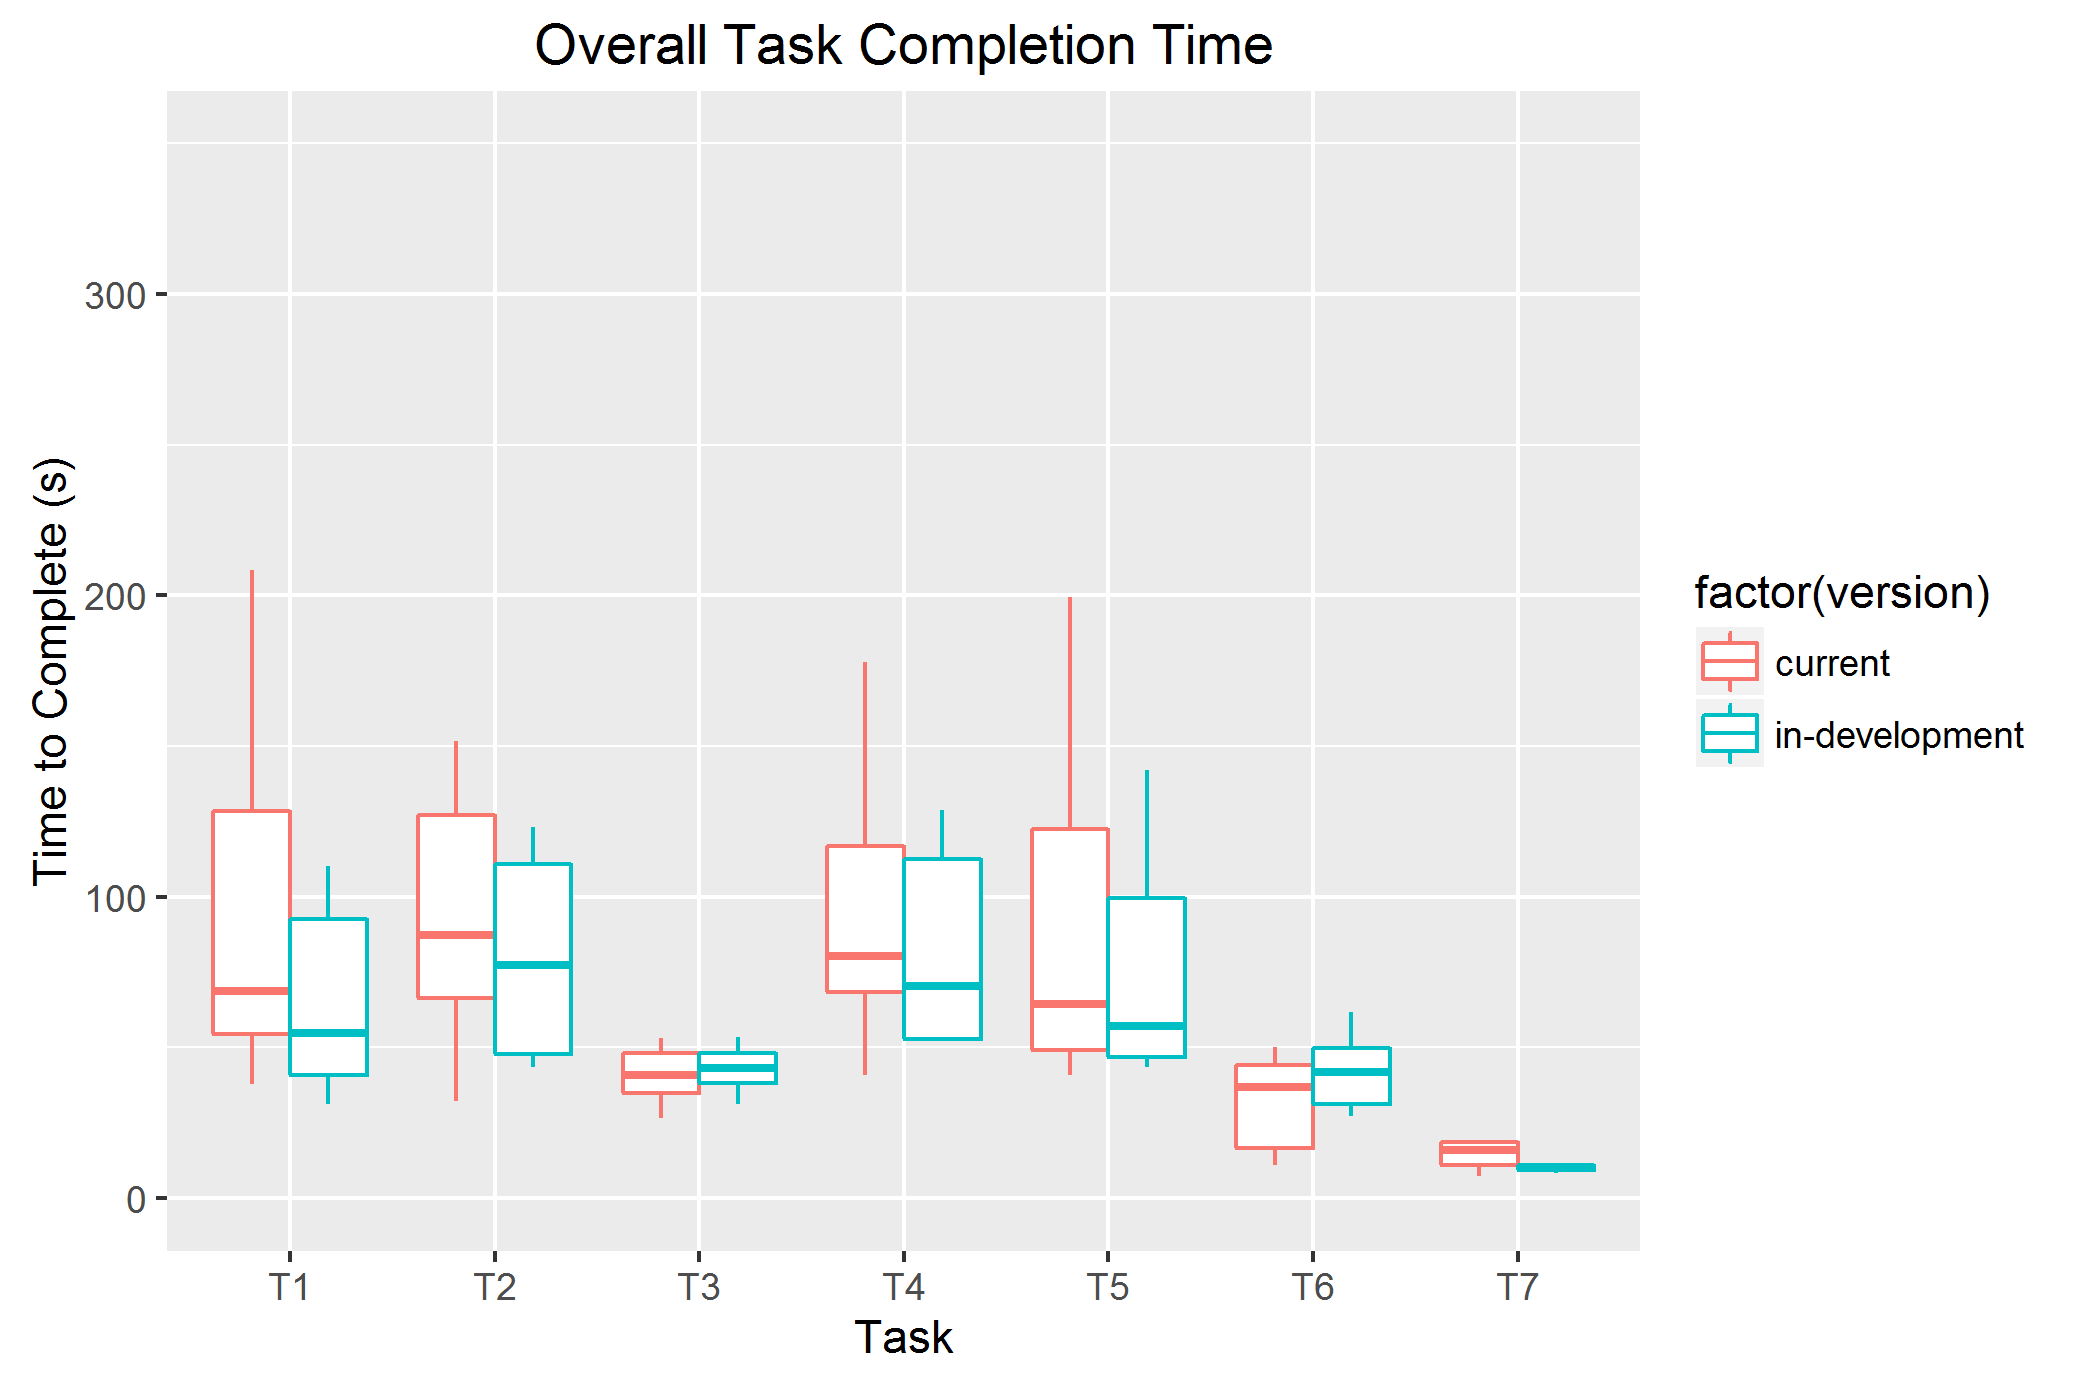
\includegraphics[width=.6\linewidth]{overall_task_completion}
  \caption{A box and whisker plot indicating the nature of the task completion times for the tasks participants were given.}
  \label{fig:overall_task_completion}
\end{figure}

On average, it appears that the \emph{in-development} version was either significantly better (in the practical, not statistical, sense) than the \emph{current} version, or at least competitive with it.

\begin{table}[h]
    \centering
    \begin{tabular}{| c | c | c | c | c | c | c | c |}
    \hline
    \multicolumn{8}{|c|}{Average Task Completion Times (s) by Task} \\
    Interface Version & T1 & T2 & T3 & T4 & T5 & T6 & T7 \\
    \hline
    \hline
    Current           & 104.0 &  93.7 &  44.3 &  95.5 & 107.9 &  37.1 &   16.1 \\
    \hline
    In-Development    & 144.4 &  79.8 &  48.2 &  93.2 &  76.9 &  45.9 &   11.9 \\
    \hline
    \hline
    Difference        & 40.4  & -13.9 &   3.9 &  -2.3 & -31.0 &   8.8 &    4.2 \\
    \hline
    \% Difference     & 38.8  & -14.8 &   8.8 &  -2.4 & -28.7 &  23.7 &   26.1 \\
    \hline
    \hline
    Significant (Y?) &        &       &       &       &       &       &       \\
    \hline
    p-Value          & 0.543  & 0.470 & 0.729 & 0.928 & 0.408 & 0.457 & 0.264 \\
    \hline
    F-Value          & 0.389  & 0.552 & 0.125 & 0.009 & 0.729 & 0.586 & 1.355 \\
    \hline
    \end{tabular}
    
    \caption{Average task completion times by interface version. Difference and percent difference is computed relative to the \emph{current} version values.}
    \label{tab:avg_task_time}
\end{table}

%
\subsubsection{Task Effort}
A variable added on suggestion of a fellow researcher was to count the clicks a participant required to complete a task, as a measure of how much searching a user does to find a target in the interface. This proved to be good advice, as it was a more stable metric than \emph{Task Performance}. It was more stable in that it was not swayed as much by a user's "processing capacity" and correlated more directly with the amount of the site a user needed to observe to learn their way around the interface.

\begin{figure}[h!]
  \centering
  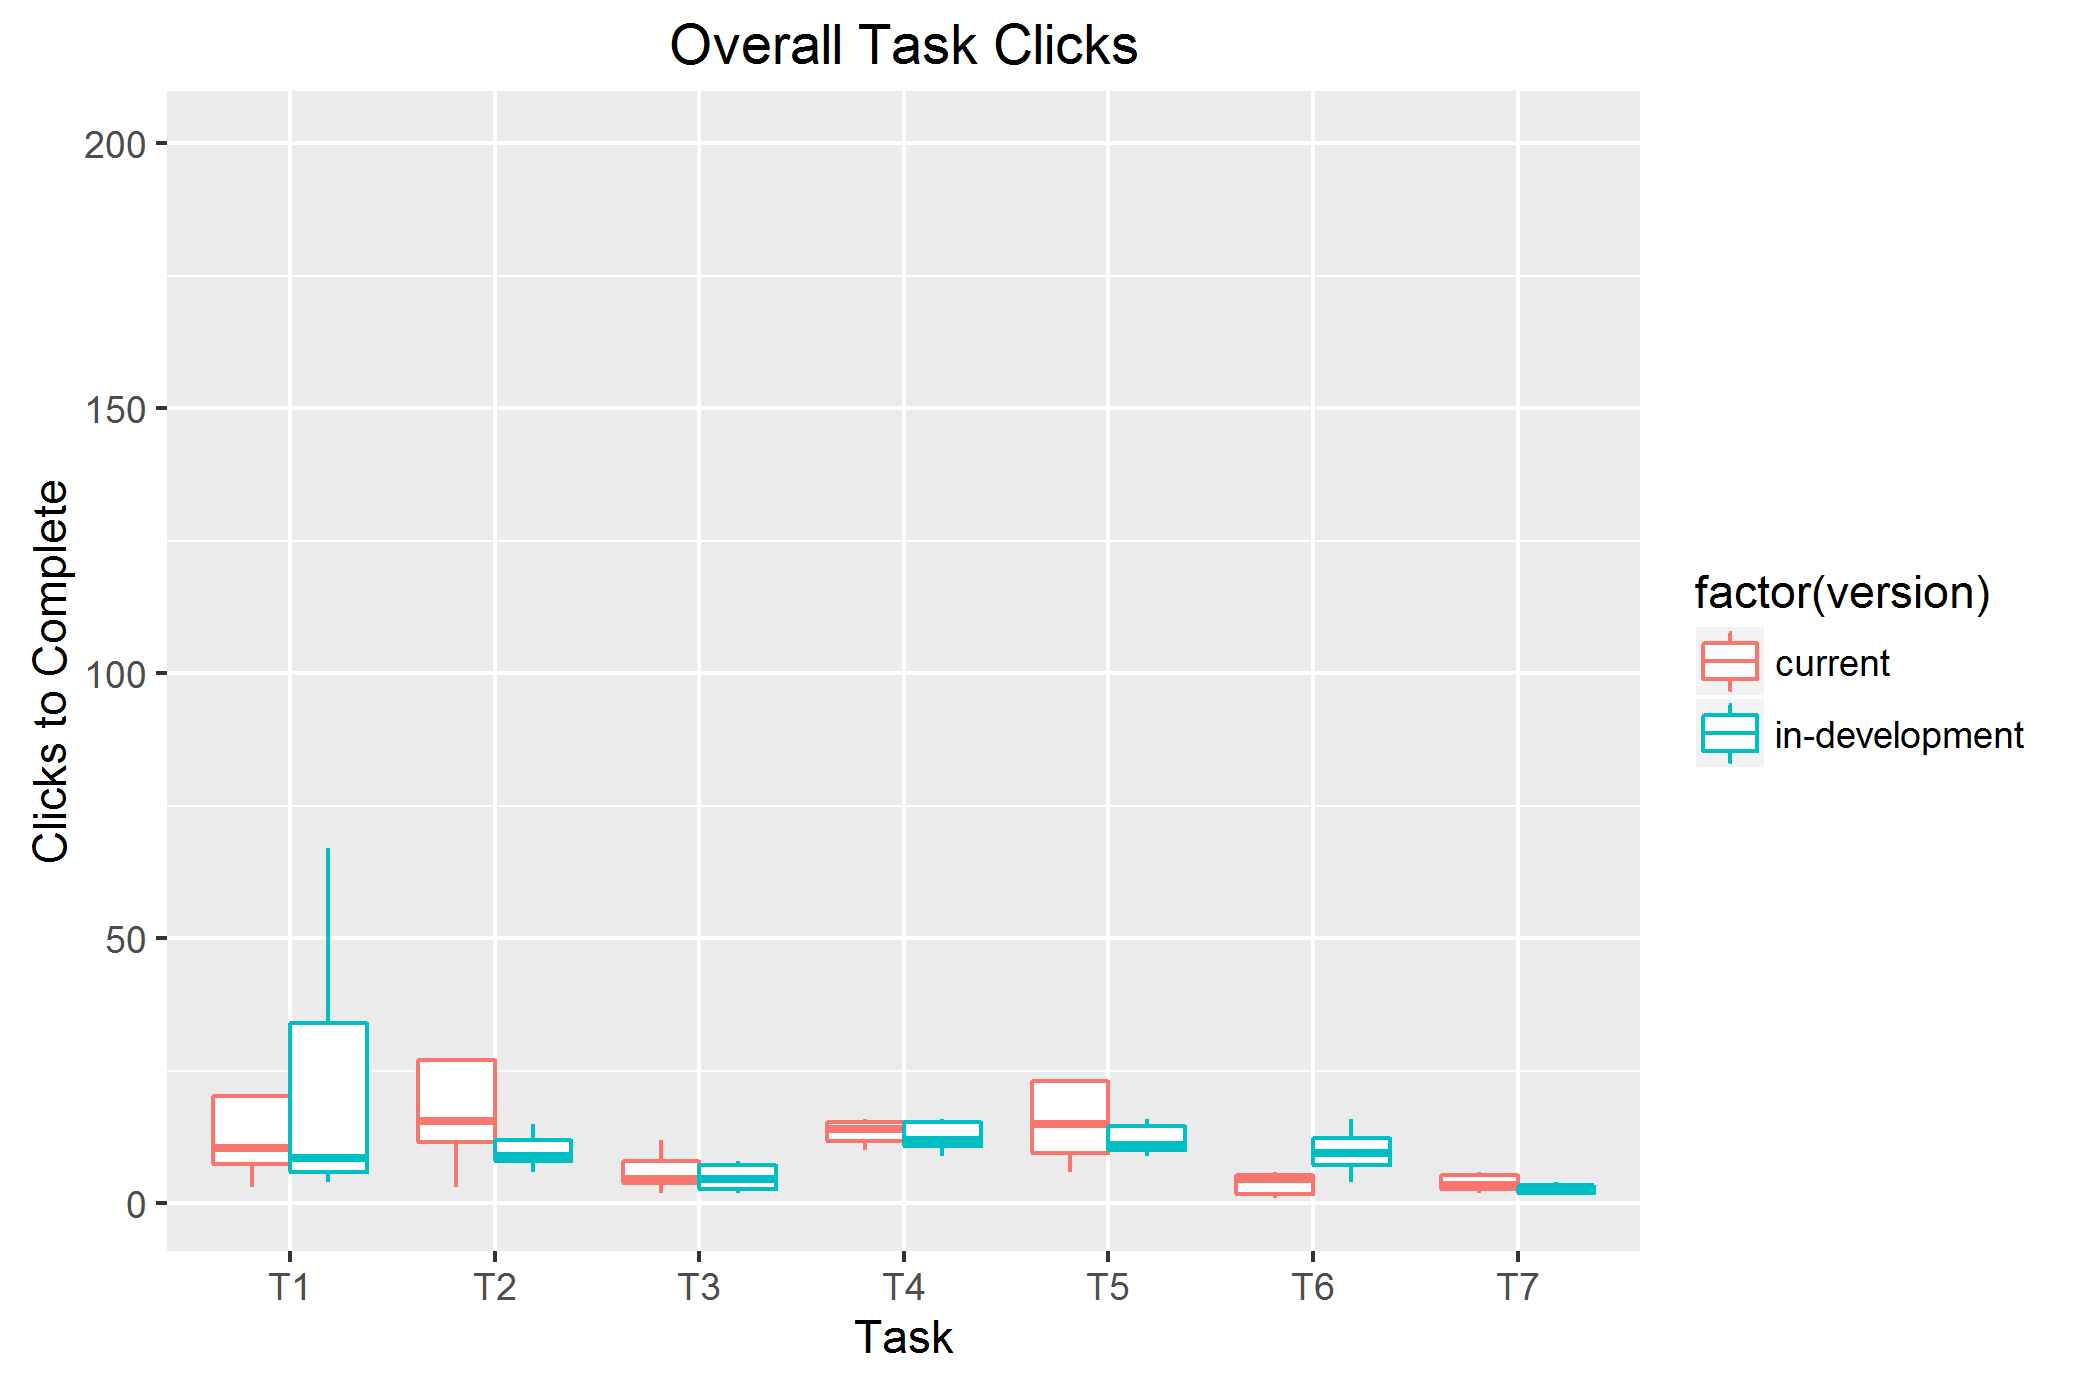
\includegraphics[width=.6\linewidth]{overall_task_clicks}
  \caption{A box and whisker plot indicating the number of clicks required to complete the tasks participants were given.}
  \label{fig:overall_task_clicks}
\end{figure}

Once again, as in \emph{Task Performance}, it appears that the \emph{in-development} version was either significantly better (in the practical, not statistical, sense) than the \emph{current} version, or at least competitive with it.

\begin{table}[h]
    \centering
    \begin{tabular}{| c | c | c | c | c | c | c | c |}
    \hline
    \multicolumn{8}{|c|}{Average Clicks to Complete a Task} \\
    Interface Version & T1 & T2 & T3 & T4 & T5 & T6 & T7 \\
    \hline
    \hline
    Current           & 36.6 & 26.0 &  6.0 & 14.3 & 15.4 &  4.5 &  4.8 \\
    \hline
    In-Development    & 28.6 & 10.8 &  6.4 & 16.6 & 13.9 &  9.6 &  3.5 \\
    \hline
    \hline
    Difference        & -10.0 & -15.2 & 0.4 & 2.3 & -1.5 &  5.1 &  -1.3 \\
    \hline
    \% Difference     & -27.3 & -58.5 & 6.7 & 16.1 & -9.7 & 113.3 & -27.1 \\
    \hline
    \hline
    Significant (Y?) &       &       &       &       &       &     Y &       \\
    \hline
    p-Value          & 0.773 & 0.191 & 0.882 & 0.625 & 0.678 & 0.018 & 0.425 \\
    \hline
    F-Value          & 0.086 & 1.885 & 0.023 & 0.250 & 0.180 & 7.215 & 0.676 \\
    \hline
    \end{tabular}
    
    \caption{Average task completion times by interface version. Differences and Percent Differences are computed relative to the \emph{current} version values.}
    \label{tab:avg_clicks}
\end{table}

%
\subsubsection{Task Perseverance}
Much to our surprise, \emph{Task Perseverance} was uninformative. We underestimated the perseverance levels the participants might have in general. Participants just gave up too rarely to allow us to discern any kind of effect. However, this is good news, because it indicates that the NRDC is not so hard that people give up (in any version).

\begin{table}[h]
    \centering
    \begin{tabular}{| c | c | c | c | c | c | c | c |}
    \hline
    \multicolumn{8}{|c|}{Total Task "Give-Ups" by Task} \\
    Interface Version & T1 & T2 & T3 & T4 & T5 & T6 & T7 \\
    \hline
    \hline
    Current           &  1 &  0 &  0 &  0 &  0 &  0 &  0 \\
    \hline
    In-Development    &  1 &  0 &  0 &  0 &  0 &  0 &  0 \\
    \hline
    \end{tabular}
    
    \caption{Total number of times a task was "given-up on", by interface version. Participants were more perseverant than expected, reducing the insight conveyed by the task-perseverance variable.}
    \label{tab:give_ups}
\end{table}

%
\subsection{Qualitative}

Overall, the NRDC was received moderately well, and many supportive criticisms were given. Participants largely preferred the \emph{in-development} to the \emph{current} version of the NRDC interface. Most of their criticisms were in regards to the services themselves, and not the NRDC interface.

\begin{table}[h]
    \centering
    \begin{tabular}{| c | p{9.5cm} |}
    \hline
    \multicolumn{2}{|c|}{Common Criticisms and Observations About the NRDC} \\
    Source & Criticism/Observation \\
    \hline
    \hline
    Participant & (Referring to the current NRDC interface) "Navigation between some of the services is difficult as the nav bar disappears." \\
    \hline
    Participant & (Referring to the in-development NRDC interface and the way it presents services in the same window) "Exiting a pop up window for services may not be intuitive for some people." \\
    \hline
    Participant & "On the [geo-spatial] search, it was confusing at first as to which parts of the interface to click first, and what conditions would be needed to be met to download / visualize data." \\
    \hline
    Participant & "Keep a persistent nav bar  at top so it's always possible to get back and easy to navigate." \\
    \hline
    Participant & "I feel as though the image retrieval (the one which makes composite videos) UI throws too much information at you all at once." \\
    \hline
    Researcher  & The list drop-down for selecting locations in the geo-spatial data search should be made more prominent. \\
    \hline
    Researcher  & The links to the services in the NRDC home page should be re-ordered by relevance and be made more distinguishable from one another. \\
    \hline
    Researcher  & If the Webcam Streams are deprecated, they should be clearly marked as such or removed. \\
    \hline
    \end{tabular}
    
    \caption{A sampling of the criticisms and observations the experiment produced.}
    \label{tab:criticisms_observations}
\end{table}

\subsubsection{Navigating Between Tasks}
Much of the experiment was focused on helping users to navigate effectively and pleasantly. It was not statistically significant that users could navigate between tasks any more quickly, but the feedback on the quality of the site was more positive for the \emph{in-development} version.

Many of the participants requested that there be some kind of omni-present "nav bar" to help them navigate effectively, as there were complaints about getting lost, or being unable to return to a previous screen easily. The \emph{in-development} version sought to address this by, instead of creating a new tab, presenting the service being accessed in the same window. However, the lack of said "nav bar" or an explicit widget to close the sub-window did present minor confusion for some participants.

\subsubsection{Geo-spatial Data Search}
In general, participants suffered the largest difficulties using the Geo-spatial Data Search. There was a large number of controls and pieces of information for participants to understand, and this led to frustration for participants.

One of the most requested features was actually a list or some kind of search functionality to help users select the target location in the Geo-spatial Data Search. Interestingly, there is a list functionality for just this purpose, but few (2) of the users noticed it, indicating that it should be made more noticeable.

Also of interest is the fact that there is a video-tutorial available on the Geo-spatial Data Search page. However, none of the participants used it. We did have a test participant (not counted in the data, used to test our procedure) who did use the tutorial, but this was the only instance of tutorial use. The general thinking among participants and the researchers was that the task should be simple, and watching a video would be an annoying waste of time.

\subsubsection{Current Conditions vs. Geo-spatial Data Search}
In all task sets, the first task required the participant to use the Current Conditions service. We observed that almost all of the participants used the Geo-spatial Data Search initially instead, thinking that the Geo-spatial Data Search would provide current data along with any other data.

Likely aiding in the occurrence of this misconception was the relative positioning of the links for the Geo-spatial Data Search and the Current Conditions services. Both are located in a drop-down menu simply labeled "Data", but Current Conditions is listed further down the list. We observed participants mousing over "Current Conditions" several times and using the Geo-spatial Data Search instead.

For these reasons, we make the recommendation that items should be re-ordered, or perhaps decorated to emphasize the information they can provide to a user.

%
%
\section{Analysis of Variance and Further Discussion}

Unfortunately, many of the more objective results were not statistically significant. That being said, the more subjective results did have statistical significance, and did demonstrate that the \emph{in-development} version of the interface was preferable.

For the direct subjective comparison of the interfaces, the \emph{in-development} version of the interface was, on average, between preferable and strongly preferred. These results were statistically significant ($F_{1,8} = 4.677$, $p < 0.05$, at worst) (see \ref{tab:avg_direct_comparison}).

The average \emph{Task Performance} displayed average changes ranging from a slowdown of 38 percent to a speed up of 28 percent when comparing the \emph{current} version of the NRDC with the \emph{in-development} version. These results were not statistically significant ($F_{1,8} = 1.355$, $p > 0.264$, at best) (see table \ref{tab:avg_task_time}). Without statistical significance it is difficult to make any meaningful remarks on the effect of \emph{Interface Version}.

The average \emph{Task Effort} displayed average changes ranging from an increase in clicks required of 113 percent to a decrease in clicks of 58 percent when comparing the \emph{current} version of the NRDC with the \emph{in-development} version. These results were largely non-statistically significant ($F_{1,8} = 7.215$, $p < 0.05$, at best), with only a single task achieving significance ($F_{1,8} = 1.885$, $p > 0.191$, at best) (see table \ref{tab:avg_clicks}). Without statistical significance it is difficult to make any meaningful remarks on the effect of \emph{Interface Version}.

The lack of statistical significance in some of the data was likely due to the small number of participants. As it turned out, it took anywhere from 30 minutes to an hour per participant once one accounted for time required to find a participant, time to brief them, time for the experiment itself, and time to debrief and answer participant questions (there was a lot of interest in the NRDC). This made it difficult to process a larger number of participants.

We do not see the lack of statistical significance for the more objective results to be particularly problematic.

First, when one considers the two interface versions, the two do have strong similarities in layout and design (a choice made to avoid disrupting the workflow of current, active users). This means that it would be unreasonable to have a large expectation of performace differences.

Second, typical users often do not think about their performance in terms of task times or numbers of clicks. While it would be nice to improve these statistics, it might not necessarily have strong bearing on user satisfaction with the NRDC, which is the primary goal. Further, since the subjective results do show that users prefer the \emph{in-development} version, it affirms that the redesigns are going in a good direction that does increase user satisfaction. Perhaps future redesigns can address user task performance further.

One final thing to mention is that the tasks were highly dependent on the services of the NRDC. We did not want to focus on testing too much around the services (other than observationally) because we did not have the capability to vary attributes of the services themselves. While we do present our findings regarding the services themselves (which are largely observational), we believe that the services are strong candidates for future experimentation of this sort, and might have as much relevance on user satisfaction as the NRDC interface itself.

%
%
\section{Additional Information}
The researchers would like to acknowledge I. Scott MacKenzie\cite{hci-research-perspective} for their excellent text book on conducting empirical research, which guided the design of this experiment; Nakarada-Kordic and Lobb\cite{PerceivedAttractiveness} and Krug\cite{dontmakemethink} for their previous research on web interface usability, and Le, Neff, Stewart, Kelley, Fritzinger, Dascalu, and Harris\cite{microservice-nrdc} for their intial and continued development of the NRDC. We would also like to acknowledge our test participant, Chase Carthen, and all of the actual participants we gathered.

%
%
% \section{About the Authors}
% %
% \subsection{Terence Henriod}

% Terence is a graduate student in the Computer Science and Engineering(CSE) department at the University of Nevada, Reno (UNR). Terence previously graduated with a Bachelor's Degree in Community Health Sciences from UNR and continued his graduate studies in CSE, expecting to finish in May of 2016. Terence has worked in industry for an IoT startup (and maintains a continued interest in IoT), and is excited to begin working at GE Bently in May after graduation.

% %
% \subsection{Vinh Le}

% Vinh is a graduate student in the Computer Science and Engineering department at the University of Nevada, Reno and graduated previously with a Bachelor's Degree in CSE at the very same university. In regards to professional interests, Vinh favors development in software engineering, web technologies, and human-computer interaction.
% 
%
%

\printbibliography

\end{document}
